% $Id$

\chapter{Quick Start Tutorial}
\label{chap:tutorial}

This chapter provides a quick start tutorial for using CUTS. Before 
beginning this tutorial, you should already be familiar with the 
following technologies:
\begin{itemize}
 \item Component Integrated ACE ORB (CIAO)
 \item Component Synthesis with Model Integrated Computing (CoSMIC)
 \item Deployment And Configuration Engine (DAnCE)
\end{itemize}

The purpose of this tutorial is to give you a quick introduction 
to using CUTS. For this tutorial, you will be creating a simple 
client/server application and measuring the oneway event latency 
(\textit{i.e.}, measuring how long it takes an event to travel between 
two components). At the end of this tutorial, you will have a basic 
understanding of the following:
\begin{itemize}
 \item Add simple behavior to a component. This is discussed in
 Section~\ref{sec:tutorial-behavior}.
 
 \item Generate source code for the components for emulation. This 
 is discussed in Section~\ref{sec:tutorial-generation}.

 \item Run a CUTS emulation on a single host. This is discussed
 is Section~\ref{sec:tutorial-execution}.
 
 \item Analyze the system execution traces generated by the 
 emulation using UNITE. This is discussed in 
 Section~\ref{sec:tutorial-analysis}.
\end{itemize}

\section{Modeling Behavior and Workload}
\label{sec:tutorial-behavior}

Adding behavior and workload to a PICML model is done using two 
domain specific modeling langauges (DSMLs) named the 
\textit{Component Behavior Modeling Language (CBML)} and the 
\textit{Workload Modeling Language (WML)}, respectively. Both 
DSMLs have been integrated into PICML so users can reference 
the structural model of their systems when modeling the system's 
behavior and workload.

Before we begin adding behavior client/server example, we first 
need the following file into GME:
\begin{lstlisting}
$(CUTS_ROOT)/tutorials/QuickStart/models/QuickStart.xme
\end{lstlisting}

\noindent Right now, behavior and workload modeling is supported 
at the component level. In this example, we will be adding behavior the 
\texttt{PingComponent}, which is located at 
\texttt{InterfaceDe\-fi\-ni\-tions/PingPong/PingPong}. In 
this tutorial, we have already added behavior and workload to 
the \texttt{PongComponent} since it is more complex.

\subsubsection{The PingComponent Behavior}

This PingComponent already contain model elements for its output 
port. What remains is associating the correct behavior and workload 
with this output port for emulation purposes. With this in mind, 
we are going to assume the PingComponent sends periodic events to 
the any component connected to its output port. Therefore complete 
the following steps (elements will be automatically be generated 
as well):
\begin{enumerate}
  \item Add a \texttt{PeriodicTask} model element to the active model 
  and set its name to eventProducer and its \texttt{Hertz} attribute 
  to 10 (\textit{i.e.}, 10 events/sec).
    
  \item Insert an \texttt{InputAction} element, change its name to 
  \texttt{eventProducer}, and connect the \texttt{PeriodicTask} to 
  the \texttt{InputAction}.
    
  \item Insert an \texttt{OutputAction}. This will automatically 
  generate a new \texttt{State} element and connect it with the 
  inserted \texttt{OutputAction}.
    
  \item Connect the final State with the originating \texttt{InputAction}, 
  \textit{i.e.}, \texttt{periodicPing}, to signify end of the behavior.
    
  \item Insert a \texttt{Variable} model element and set it to reference 
  the \texttt{UnsignedLongInteger} element in the \texttt{PredefinedTypes} 
  folder. Name the variable \texttt{eventCount} and set the initial value 
  of the variable to 0.
    
  \item Select the connection between the \texttt{InputAction} and the 
  \texttt{State}. Type the following in the \texttt{Effects} attribute 
  field: \texttt{this->eventCount\_ ++;}
  
  \item Open the \texttt{OutputAction} and insert a \texttt{SimpleProperty}. 
  Set it to reference the \texttt{Un\-sign\-ed\-Long\-Integer} element in the 
  \texttt{PredefinedTypes} folder, and set its \texttt{Value} attribute 
  to the following: \texttt{this->eventCount\_}.
\end{enumerate}
\begin{figure}[htbp]
  \centering
  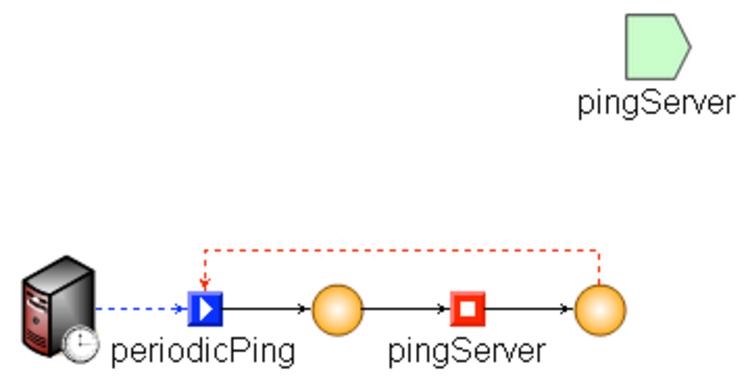
\includegraphics[scale=0.3]{gettingstarted-client-behavior.pdf}
  \caption{Complete behavior model for the PingComponent.}
  \label{fig:tutorial-behavior}
\end{figure}
Figure~\ref{fig:tutorial-behavior} illustrates the complete behavior 
model of the \texttt{PingComponent} in PICML.

\section{Generating Source Code for Emulation}
\label{sec:tutorial-generation}

After modeling the behavior and workload, the next step is to generate 
source code from the model. This will enable emulation of the test 
system on its target architecture. To generate source code from the 
model, launch the CUTS interpreter and execute the following steps:
\begin{enumerate}
  \item Enter the target output directory
  
  \item Select \textbf{Component Integrated ACE ORB (CIAO)} in the listbox
  
  \item Click the \textbf{OK} button
\end{enumerate}

Once the CUTS interpreter finishes generating source code, the IDL 
files need to be generated in order to compile the source code. 
These files are created by the IDL Generator provided with CoSMIC. 
Finally, there will be a \texttt{QuickStart.mwc} file located in the output 
directory selected for source code generation. This is a
\textit{Makefile, Project and Workspace Creator (MPC)} workspace file 
that contains 
all the necessary information to sucessfully compile the generated 
source code. Use \texttt{QuickStart.mwc} to generate the appropriate 
workspace and then compile it.

\textbf{NOTE:} The auto-generated source code for this model is 
also available at the following location: 
\begin{lstlisting}
$(CUTS_ROOT)/tutorials/QuickStart
\end{lstlisting}

\section{Running a CUTS Emulation}
\label{sec:tutorial-execution}

One design goal of CUTS is to (re)use the same infrastructure 
used in the target environment. The QuickStart example uses 
the \textit{Deployment And Configuration Engine (DAnCE)}, which 
is included with CIAO's standard distribution, to deploy the 
test system. To deploy the example, use the following steps:
\begin{enumerate}
  \item Copy the contents of the \texttt{./descriptors} directory 
  in the tutorial to the directory where you generated the source 
  code.
  
  \item In one window, launch the deployment infrastructure using 
  the following command:
\begin{lstlisting}
%> cutsnode_d -c deployment.config
\end{lstlisting}
  
  \item  In another window, launch the test using the following 
  command:
\begin{lstlisting}
%> cutstest -c test.config --time=30
\end{lstlisting}

\end{enumerate}

This will run the test for 30 seconds. While the system is executing, 
it will generate an execution trace, which will be stored in the 
test database. This execution trace is what we will analyze in the 
next, and final, step.

\section{Analyzing System Execution Traces}
\label{sec:tutorial-analysis}

CUTS analyzes quality-of-service (QoS) properties via system execution
traces with a tool called \textit{Understanding Non-functional Intentions 
 via Testing and Experimentation (UNITE)}. In this quick start tutorial, 
we generated a system execution trace that can be used to measure the 
service time of an event. We are now going to use UNITE to analyze 
the generated system execution trace. To do this, execute the following 
steps:
\begin{enumerate}
  \item Copy the contents of the \texttt{./analysis} directory in the 
  tutorial to the directory where you generated the source code.
  
  \item Execute the following command:
\begin{lstlisting}
%> cuts-unite -f ../descriptors/00000000-0000-0000-0000-000000000000.cdb 
  -c QuickStart.unite
  \end{lstlisting}
\end{enumerate}

After executing UNITE, you should get an average service time for an 
event based on what is captured in the generated system execution 
trace.

